\chapter{Oasis Lib}
\label{ch:Lib}
In this chapter we describe the library of the administration module, called Oasis Lib. The Oasis Lib is the library, which works as a connection between the Oasis Local Db (\vref{ch:Db} and the applications, which runs on the GIRAF system, by providing an API, which the GIRAF applications can use. First the structure of Oasis Lib is described in section \vref{sec:Structure}. Then how the Oasis Lib is implemented is described in section \vref{sec:LibImp}.

\section{Structure}
\label{sec:Structure}
In the structure of Oasis Lib, we have taken inspiration of the MVC pattern, where the system is divided into three parts; Model, View, and Controller. In Oasis Lib the Model part is a package containing model objects. Each model object represent a table in the local db. The model objects is used to encapsulate the data, which is supposed to be saved and loaded from the Oasis Local Db. The reason that we use model objects is to ease it for the users and to make a uniform way of saving and loading data. The controller part is the package containing all the methods, which the developers can use to interact with Oasis Local Db. We do not have any view part. This is missing because we see it as a part of the GIRAF applications.

\section{Implementation}
\label{sec:LibImp}
The Oasis Library's controllers is what make up the main part of the library. It is devided into a number of different sub controllers, the public ones seen in figure \vref{controllers}.

\begin{figure}
	\centering
		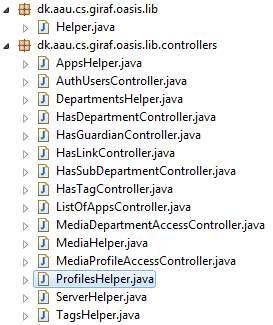
\includegraphics[width=\textwidth]{images/controllers.png}
	\caption{The different controlers in Oasis library}
	\label{fig:controllers}
\end{figure}


There are a number of other sub controllers as well, but they are only for internal use within the Oasis library.
For futher information on how the Oasis library's methods work, see JavaDoc REF!.